\begin{figure*}[!ht]
\centering

\begin{tikzpicture}[node distance=12mm and 14mm, every node/.style={font=\small}]

% row 1
\node[box] (trending_project) {\faGithub\ 1K GitHub\\Trending Java Projects};
\node[box,right=1.5cm of trending_project] (comments) {\faComments\ 1.6 millions test\\code comments};
\node[box,right=2cm of comments] (analyzed_comments) {\faUserCheck\ 50K manually\\analyzed comments};
\node[box,right=1.8cm of analyzed_comments] (satd_comments) {\faComments\ 615 SATD\\comments};
\node[box, below=1.1cm of satd_comments] (classified_satd) {\faChartBar\ \categoryCount{} types of SATD};

% RQ branch (final row)
\node[smallbox, below=22mm of analyzed_comments, xshift=-30mm] (rq2) {\faSearch\ Detect with\\existing tool};
\node[smallbox, below=22mm of analyzed_comments] (rq3) {\faBrain\ Detect with\\ open-source LLMs};
\node[smallbox, below=22mm of analyzed_comments, xshift=30mm] (rq4) {\faLock\ Detect with\\proprietary LLMs};

% arrows row1 -> row1 (horizontal)
\draw[arrow] (trending_project) -- (comments) 
    node[midway, above, arrowicon]{\faTools} 
    node[midway, below, align=center]{extract\\comments};
\draw[arrow] (comments) -- (analyzed_comments) 
    node[midway, above, arrowicon]{\faRandom}
    node[midway, below, align=center]{randomly\\select and analyze};
\draw[arrow] (analyzed_comments) -- (satd_comments)
    node[midway, above, arrowicon]{\faFilter}
    node[midway, below, align=center]{filter};

\draw[arrow] (satd_comments) -- (classified_satd)
    node[midway, left, arrowicon]{\faUsers}
    node[midway, right, align=center]{RQ1\\manually\\classify};

% vertical drop then horizontal branch
\coordinate (branch) at ($(analyzed_comments.south)+(0,-1cm)$);

% \draw[arrow] (analyzed_comments.south) -- (branch)
%     node[midway, left, arrowicon]{\faArrowDown}
%     node[midway, right]{automated detection};
\draw[semithick] (analyzed_comments.south) -- (branch)
    node[midway, left, arrowicon]{\faRobot}
    node[midway, right, align=center]{automated detection};

% horizontal arrows to RQ boxes
\draw[arrow] (branch) -| (rq2.north)
    % node[pos=0.3, above, arrowicon]{\faChartBar}
    node[pos=0.3, below, align=center]{RQ2};
\draw[arrow] (branch) -- (rq3.north)
    % node[midway, left, arrowicon]{\faRobot}
    node[midway, right]{RQ3};
\draw[arrow] (branch) -| (rq4.north)
    % node[pos=0.3, above, arrowicon]{\faUserCheck}
    node[pos=0.3, below]{RQ4};

\end{tikzpicture}

\caption{Workflow for collecting, sampling, analyzing, classifying test code comments (RQ1), and evaluating automated SATD detection using existing tools (RQ2), open-source LLMs (RQ3), and proprietary LLMs (RQ4).}
\label{fig:methodology}
\end{figure*}


\section{Methodology}

\label{sec:methodology}
Figure~\ref{fig:methodology} presents a high-level overview of our overall methodology, outlining the key stages involved in data collection, comment extraction, manual labeling, and SATD detection using both traditional and LLM-based approaches. It also clarifies how each branch maps to our research questions: manual taxonomy construction in RQ1 and automated detection pipelines in RQ2--RQ4.


\subsection{Project Selection}
We aimed to collect comments from a diverse range of projects to avoid relying on a limited set of contributors, which could hinder the generalizability of our observations. Such generalizability is essential for developing a benchmark dataset, as selecting SATD from only a few projects would be strongly influenced by the commenting styles of a small number of individuals. This, in turn, would hinder the meaningful evaluation of current and future SATD detection tools. 
While selecting a large number of projects, however, we had to ensure that the collected comments were not predominantly drawn from low-quality projects (e.g., toy projects)~\cite{kalliamvakou_promises_2014}. Therefore, we used GitHub’s trending project list, ranked by the number of stars retrieved via the GitHub API. Although Borges et al.~\cite{borges_whats_2018} showed that star counts do not always correspond to sustained engagement or project quality, they also found that many practitioners continue to consider star counts before adopting a tool in their projects. Nevertheless, we mitigated the potential negative impact of star-based project selection by including another popularity indicator---we did not include projects with fewer than 100 forks. In addition, we randomly analyzed 100 projects and found that the selected repositories were well-maintained. 

At the end, we selected 1,000 Java-based repositories that were more likely to contain meaningful discussions and development practices relevant to our study. We focused on a single programming language only due to reliance on a parser for comment extraction—supporting multiple programming languages would require multiple parsers. Also, since our focus is on test code only, we needed techniques to exclude production code files (described in Section~\ref{sec:comment-parsing}), which would have been more challenging if applied across multiple programming languages. The selected projects cover a wide range of software types, including libraries, frameworks, applications, and middleware. Figure \ref{fig:repository_statistics} shows the distribution of stars, forks, watchers, commits, and extracted test code comment counts across these projects.
% , \textcolor{red}{while the complete list can be accessed here}.\footnote{\url{\repositoryUrl/data/repository.csv}}
%including number of comments analyzed, SATD.


\begin{figure*}[!ht]
\centering
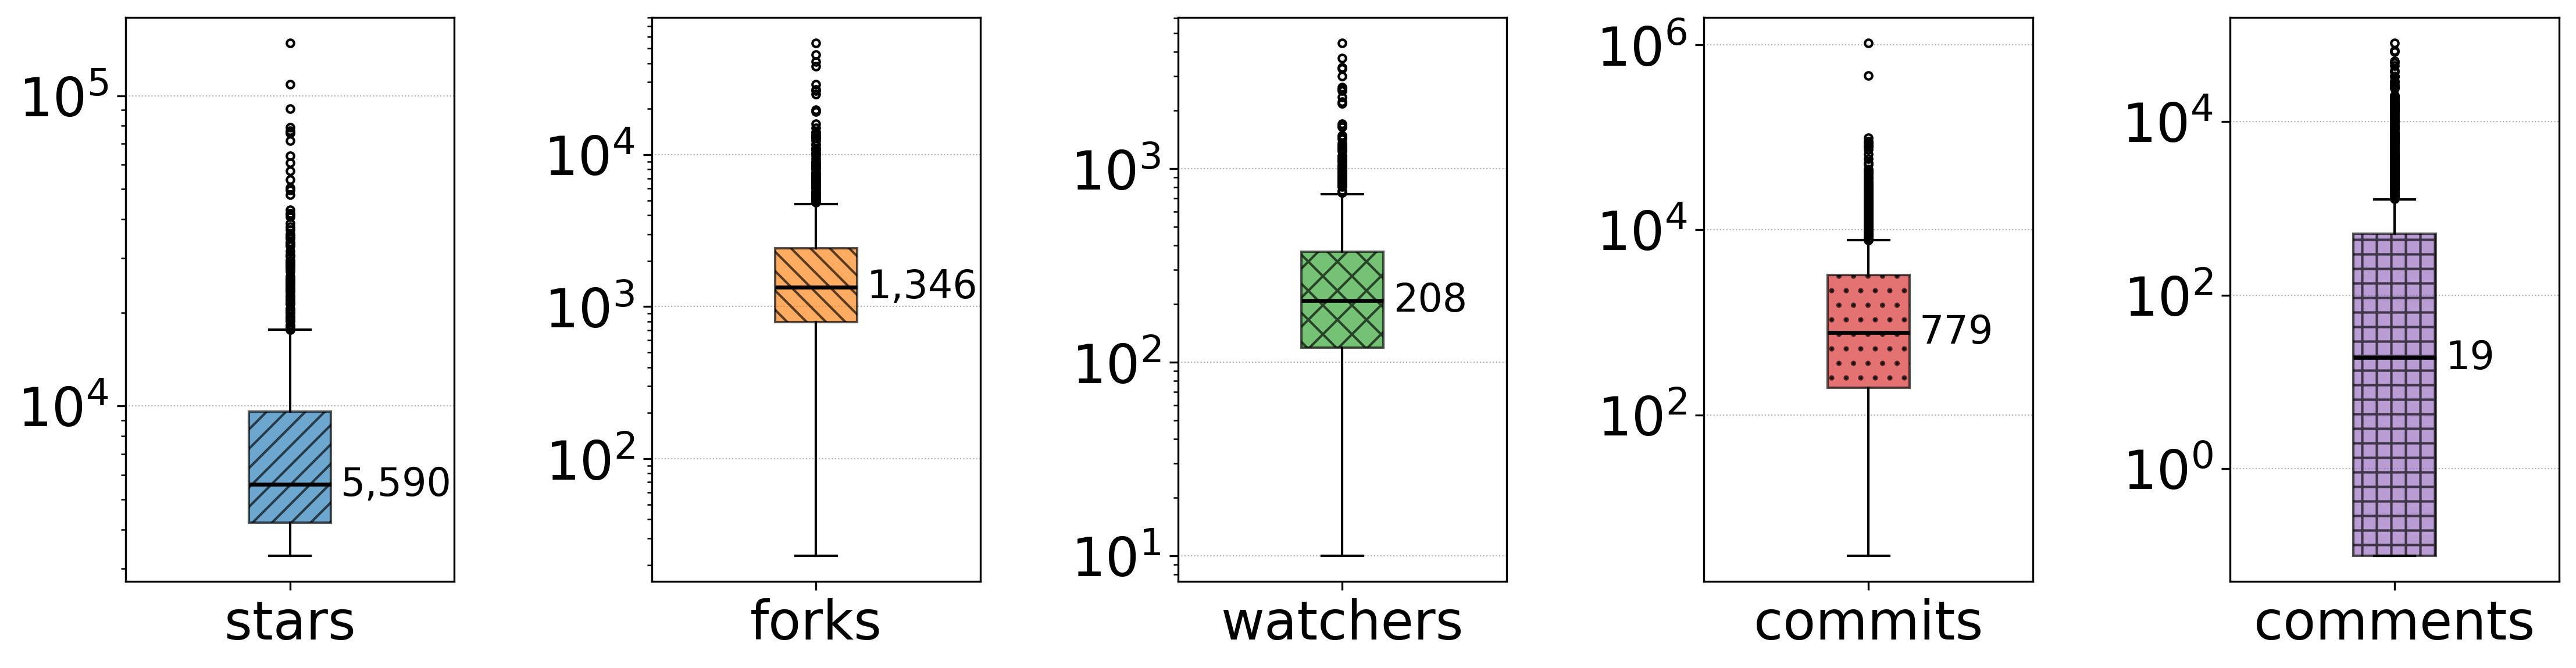
\includegraphics[width=\textwidth]{figure/repository_statistics.jpg}
\caption{Distribution of stars, forks, watchers, commits, and the number of extracted test code comments across the selected projects.}
\label{fig:repository_statistics}
\end{figure*}

% \begin{table}[ht!]
\centering
\caption{50 sample projects among a total of 1,000 projects.}
\label{table:top_well_known_projects}
\resizebox{\linewidth}{!}{
\begin{tabular}{lrrrrr}
\toprule
\textbf{Name} & \textbf{Stars} & \textbf{Forks} & \textbf{Watchers} & \textbf{Comments} \\
\midrule
Apktool & 21,269 & 3,653 & 21,269 & 101 \\
aws-sdk-java & 4,147 & 2,823 & 4,147 & 1,364 \\
butterknife & 25,561 & 4,598 & 25,561 & 53 \\
dagger & 7,299 & 3,070 & 7,299 & 114 \\
dbeaver & 41,691 & 3,564 & 41,691 & 247 \\
elasticsearch & 71,573 & 25,041 & 71,573 & 43,420 \\
eureka & 12,485 & 3,760 & 12,485 & 474 \\
EventBus & 24,720 & 4,668 & 24,720 & 94 \\
fastjson & 25,777 & 6,497 & 25,777 & 3,223 \\
flink & 24,507 & 13,505 & 24,507 & 32,963 \\
groovy & 5,255 & 1,897 & 5,255 & 153 \\
grpc-java & 11,580 & 3,872 & 11,580 & 6,703 \\
gson & 23,544 & 4,300 & 23,544 & 961 \\
guava & 50,499 & 10,950 & 50,499 & 551 \\
hadoop & 14,931 & 8,936 & 14,931 & 65,223 \\
HikariCP & 20,241 & 2,964 & 20,241 & 655 \\
hive & 5,623 & 4,709 & 5,623 & 19,117 \\
Hystrix & 24,230 & 4,722 & 24,230 & 2,042 \\
intellij-community & 17,643 & 5,345 & 17,643 & 2,723 \\
javaparser & 5,675 & 1,184 & 5,675 & 2,795 \\
jdk & 20,386 & 5,695 & 20,386 & 46,941 \\
jedis & 11,969 & 3,879 & 11,969 & 3,033 \\
jenkins & 23,601 & 8,925 & 23,601 & 4,074 \\
jmeter & 8,564 & 2,137 & 8,564 & 1,330 \\
junit4 & 8,528 & 3,279 & 8,528 & 262 \\
junit5 & 6,508 & 1,518 & 6,508 & 7,133 \\
kafka & 29,425 & 14,162 & 29,425 & 19,748 \\
libgdx & 23,719 & 6,458 & 23,719 & 179 \\
lombok & 13,037 & 2,417 & 13,037 & 17 \\
mockito & 15,017 & 2,583 & 15,017 & 2,587 \\
mybatis-3 & 19,943 & 12,899 & 19,943 & 1,841 \\
neo4j & 13,780 & 2,414 & 13,780 & 23,952 \\
netty & 33,769 & 16,012 & 33,769 & 5,557 \\
presto & 16,194 & 5,411 & 16,194 & 12,907 \\
pulsar & 14,431 & 3,611 & 14,431 & 15,524 \\
questdb & 14,881 & 1,207 & 14,881 & 8,327 \\
rocketmq & 21,502 & 11,757 & 21,502 & 1,760 \\
RxAndroid & 19,865 & 2,947 & 19,865 & 28 \\
RxJava & 48,008 & 7,605 & 48,008 & 4,033 \\
selenium & 31,554 & 8,325 & 31,554 & 1,033 \\
spark & 9,655 & 1,564 & 9,655 & 114 \\
spring-boot & 76,104 & 40,906 & 76,104 & 6,726 \\
spring-framework & 57,294 & 38,337 & 57,294 & 13,815 \\
spring-security & 8,968 & 5,975 & 8,968 & 10,717 \\
tomcat & 7,705 & 5,095 & 7,705 & 5,692 \\
WxJava & 30,502 & 8,754 & 30,502 & 1,291 \\
zipkin & 17,118 & 3,101 & 17,118 & 1,163 \\
zookeeper & 12,372 & 7,260 & 12,372 & 4,127 \\
zuul & 13,619 & 2,405 & 13,619 & 385 \\
zxing & 33,050 & 9,376 & 33,050 & 794 \\
\bottomrule
\end{tabular}
}
\end{table}

% TODO
% [6, 8, 11, 13, 15, 17, 21, 28, 32, 40, 51, 53, 59, 60, 61, 63, 67, 69, 74, 81, 83, 86, 144, 173, 182]
% Trending page link
% Collect SLOC and Contributor from https://openhub.net/
\subsection{Comment Parsing}
\label{sec:comment-parsing}
The source code of each project was first retrieved from GitHub with an automated script. Since this study focuses solely on test code, it is necessary to distinguish comments in production code from those in test code. To identify test code, we leveraged two heuristics. First, as is common in Java projects using Maven, Gradle, or Ant build systems, test code files and packages are typically placed under the src/test/java directory. Therefore, all Java files within this directory were treated as test code. Second, for files located outside the standard test directory, we checked for the presence of unit test annotations (e.g., @Test, @Before) from well-known unit testing frameworks such as JUnit, Mockito, and TestNG.

For code parsing, we used JavaParser\footnote{https://github.com/javaparser/javaparser last accessed: Oct 01, 2025} to extract all associated comments—including block, line, and Javadoc types—along with their start and end line numbers. To preserve the continuity of comments, we concatenated consecutive single-line comments. This is important because developers often use multiple single-line comments to document a single concept, and failing to merge them would result in fragmented sentences and a loss of contextual meaning. As a result, the raw number of extracted comments does not directly correspond to the number of semantically distinct comments. After merging consecutive single-line comments, we obtained a total of 1,653,658 test code comments, which were stored in a relational database to enable efficient downstream processing. Among the 1,000 analyzed projects, 45 contained a substantial number of comments, each exceeding 10,000. An additional 140 projects had between 1,000 and 10,000 comments, while 497 projects had fewer than 1,000 comments. The remaining 318 projects contained no test code comments at all.

\subsection{Dataset Creation}
Since manually reviewing more than 1.6 million test comments to identify SATD comments will be extremely time-consuming, we randomly selected 50,000 comments. Similar to the original SATD study~\cite{potdar_exploratory_2014}, the first author, a graduate student with 10+ years of industry experience as a lead software engineer, checked how many of these comments are SATD, making two classes of comments: SATD and non-SATD. This process required approximately 165 hours to complete. To assess labeling reliability, we conducted an independent double-check using a statistically grounded sample targeting a 95\% confidence level. The first author provided the second author with 619 randomly selected comments, obtained through stratified sampling across the two classes (237 SATD and 382 non-SATD). The second author, another graduate student with 2+ years of industry experience as a software engineer, independently labeled these 619 samples. The Cohen's kappa coefficient~\cite{cohen_coefficient_1960} was 0.95, implying an almost perfect~\cite{viera2005understanding} inter-rater agreement score and the reliability of our dataset labeling.   

% As some projects contain more comments than others, the 50,000 randomly selected comments are not the same for each project. Table~\ref{table:top10_project_ranked_by_reviewed_comments} shows the top 50 projects (ranked by total number of reviewed comments), in addition to the number and percentage of SATD comments of the analyzed comments. 

Our manual review identified 1,024 SATD comments. However, among these 1,024 SATD comments, a striking 409 originated from a single project, OpenAPI Generator, accounting for approximately 38\% of that project’s comments. Upon closer inspection, we found that this repository contains hundreds of autogenerated Java client samples (e.g., OkHttp, Retrofit) with templated SATD comments following the pattern \textit{TODO}. Because this project disproportionately skewed the overall distribution of SATD across projects, including its comments would have hindered the generalizability of our benchmark dataset. For example, the taxonomy of SATD developed in this paper (RQ1) would be affected, and any evaluation of SATD detection tools would be biased. 
Consequently, we excluded all 1,063 comments from this project from our experimental dataset. We then removed 943 non-English comments. The refined dataset ultimately comprises 47,994 comments from 488 distinct projects, of which 615 (1.28\%) are classified as SATD, originating from 146 projects.

% updated description with number of comments of project Open AI
% \textcolor{red}{50000-409-947 = 48644, the math is not working
% Total  : 50,000
% Open AI : 1,063
% non-ASCII: 947
% Open AI non-ASCII : 4
% So 50,000 - 1,063 - 947 + 4 = 47,994
% }
%Subsequently, the comments were manually classified (RQ1) into 15 well-defined categories.

% % \begin{table}[!ht]
% \centering
% \caption{Top 10 of 1,000 projects ranked by the number of manually reviewed comments.}
% \label{table:top10_project_ranked_by_reviewed_comments}
% \resizebox{\linewidth}{!}{
% \begin{tabular}{lcc}
% \toprule
% \textbf{Project} & \makecell{\textbf{Total Comments} \\ \textbf{(Reviewed)}}& \makecell{\textbf{SATD} \\ \textbf{Comments (\%)}} \\
% \midrule
% ignite & 80,087 (2,431) & 7 (0.29)\\
% platform\_frameworks\_base & 63,155 (1,949) & 17 (0.87)\\
% hadoop & 65,223 (1,935) & 10 (0.52)\\
% camunda-bpm-platform & 49,253 (1,398) & 2 (0.14)\\
% jdk & 46,941 (1,392) & 15 (1.08)\\
% elasticsearch & 43,420 (1,304) & 37 (2.84)\\
% j2objc & 38,558 (1,194) & 27 (2.26)\\
% camunda & 36,650 (1,133) & 1 (0.09)\\
% openapi-generator & 33,297 (1,063) & 409 (38.48)\\
% camel & 32,845 (990) & 8 (0.81)\\

% \bottomrule
% \end{tabular}
% }
% \end{table}


\begin{table}[!ht]
\centering
\caption{Top 50 of 1,000 projects ranked by the number of manually reviewed comments, showing the total number of comments, reviewed comments, SATD comment count (\#), and the percentage of SATD comments (\%).}
\label{table:top10_project_ranked_by_reviewed_comments}
\resizebox{\linewidth}{!}{
\begin{tabular}{lrrrr}
\toprule
\multirow{2}{*}{\textbf{Project}} & \multicolumn{2}{c}{\textbf{Comments}} &  \multicolumn{2}{c}{\textbf{SATD}}\\
\cmidrule(lr){2-3} \cmidrule(lr){4-5}

& \textbf{Total} & \textbf{Reviewed} & \textbf{\#} & \textbf{\%} \\

\midrule
ignite & 80,087 & 2,431 & 7 & 0.29 \\
platform_frameworks_base & 63,155 & 1,949 & 17 & 0.87 \\
hadoop & 65,223 & 1,935 & 10 & 0.52 \\
camunda-bpm-platform & 49,253 & 1,398 & 2 & 0.14 \\
jdk & 46,941 & 1,392 & 15 & 1.08 \\
elasticsearch & 43,420 & 1,304 & 37 & 2.84 \\
j2objc & 38,558 & 1,194 & 27 & 2.26 \\
camunda & 36,650 & 1,133 & 1 & 0.09 \\
openapi-generator & 33,297 & 1,063 & 409 & 38.48 \\
camel & 32,845 & 990 & 8 & 0.81 \\
flink & 32,963 & 987 & 12 & 1.22 \\
hibernate-orm & 29,108 & 912 & 21 & 2.30 \\
ghidra & 27,808 & 837 & 15 & 1.79 \\
OpenSearch & 26,486 & 782 & 9 & 1.15 \\
neo4j & 23,952 & 759 & 2 & 0.26 \\
geoserver & 24,540 & 746 & 12 & 1.61 \\
hbase & 25,085 & 735 & 6 & 0.82 \\
kafka & 19,748 & 632 & 4 & 0.63 \\
flowable-engine & 18,820 & 609 & 0 & 0.00 \\
hive & 19,117 & 605 & 4 & 0.66 \\
trino & 19,979 & 587 & 22 & 3.75 \\
bazel & 19,403 & 587 & 14 & 2.39 \\
automq & 18,447 & 577 & 3 & 0.52 \\
jetty.project & 17,079 & 533 & 14 & 2.63 \\
hazelcast & 17,579 & 529 & 6 & 1.13 \\
closure-compiler & 15,307 & 508 & 28 & 5.51 \\
cassandra & 14,866 & 461 & 5 & 1.08 \\
pulsar & 15,524 & 459 & 3 & 0.65 \\
ExoPlayer & 16,246 & 455 & 6 & 1.32 \\
druid & 14,589 & 440 & 8 & 1.82 \\
beam & 15,970 & 436 & 16 & 3.67 \\
graal & 13,743 & 429 & 2 & 0.47 \\
pinot & 13,646 & 414 & 5 & 1.21 \\
iceberg & 13,141 & 413 & 4 & 0.97 \\
iotdb & 12,315 & 400 & 7 & 1.75 \\
keycloak & 12,956 & 389 & 3 & 0.77 \\
spring-framework & 13,815 & 385 & 3 & 0.78 \\
presto & 12,907 & 378 & 6 & 1.59 \\
vespa & 11,865 & 365 & 6 & 1.64 \\
incubator-kie-drools & 10,743 & 350 & 6 & 1.71 \\
openj9 & 11,239 & 347 & 6 & 1.73 \\
spring-security & 10,717 & 338 & 0 & 0.00 \\
hudi & 10,265 & 327 & 1 & 0.31 \\
quarkus & 9,583 & 304 & 3 & 0.99 \\
druid & 10,094 & 301 & 12 & 3.99 \\
springdoc-openapi & 10,075 & 291 & 0 & 0.00 \\
nifi & 9,214 & 274 & 1 & 0.36 \\
starrocks & 8,763 & 271 & 6 & 2.21 \\
calcite & 8,743 & 262 & 3 & 1.15 \\
mockserver & 8,059 & 238 & 0 & 0.00 \\
\bottomrule
\end{tabular}
}
\end{table}

We also found that our filtered dataset of 47,994 comments contains 15,439  duplicate comments---unsurprising given practitioners often use similar keywords to indicate SATD~\cite{potdar_exploratory_2014}. Therefore, we created a second dataset applying deduplication. This allows us to better evaluate the model’s ability to make predictions on completely unseen comments. Thus, the original dataset (the duplicate set) preserves the natural distribution of comments as found in the projects, while the latter dataset allows us to evaluate detection effectiveness without the risk of any data leakage. Clearly, and unsurprisingly, our dataset is highly imbalanced, with SATD instances comprising only 1.28\% of the total data. As we show later, this severe imbalance makes accurate detection particularly challenging. 

Some of our evaluations in RQ2 involve retraining the existing tools. As such, we aimed to divide the dataset into 80\% training and 20\% testing. To prevent data leakage, we ensured that each project appeared exclusively in either the training or testing set, while also maintaining the proportional distribution of SATD and non-SATD comments across both sets---i.e., 20\% of all SATD should be in the test, and the rest in the train dataset. To do so,  we constructed the test set by randomly selecting one project at a time, measuring the distributions until approximately 20\% of the total SATD and 20\% of total non-SATD comments were included. The remaining comments formed the training set. Because of project-wise selection, the split between training and testing was not always exactly 80/20, but it was very close. The details of these datasets are shown in Table~\ref{table:satd_detection_dataset}. In addition, for RQ2, we applied 5-fold cross-validation with stratified group-based splitting at the project level. This approach prevents data leakage~\cite{chowdhury_method-level_2024, pascarella_performance_2020} by ensuring that all samples from the same project remain within the same fold; thus, a project included in the training set cannot appear in the test set.


\begin{table*}[!ht]
\centering
\caption{Training and testing datasets. Percentages in parentheses indicate the proportion within the corresponding datasets. Please note that, to enable fair comparisons across all tools and approaches, all accuracy metrics in all RQs were reported using only the test dataset.}
\label{table:satd_detection_dataset}
\begin{adjustbox}{max width=\textwidth}
\begin{tabular}{llrrrrr}
\toprule
\textbf{Distribution} & \textbf{Dataset}  & \textbf{Comments (\%)}& \makecell{\textbf{non-SATD} \\ \textbf{Comments (\%)}} &  \makecell{\textbf{SATD} \\ \textbf{Comments (\%)}} & \makecell{\textbf{Overall} \\ \textbf{SATD \%}} & \textbf{Projects (\%)}\\
\midrule

Original & Train & 38,380 (80.0) & 37,902 ( 80.0) & 478 (77.7) & 1.2 & 382 (78.3) \\
Original & Test & 9,614 (20.0) & 9,477 ( 20.0) & 137 (22.3) & 1.4 & 108 (22.1) \\
Deduplicate & Train & 26,024 (79.9) & 25,621 ( 80.0) & 403 (78.1) & 1.5 & 368 (79.0) \\
Deduplicate & Test & 6,531 (20.1) & 6,418 ( 20.0) & 113 (21.9) & 1.7 & 98 (21.0) \\


\bottomrule
\end{tabular}
\end{adjustbox}
\end{table*}


\subsection{Evaluation Metrics}

To evaluate SATD detection for RQ2–RQ4, we used Precision, Recall, and F1-score following prior SATD research~\cite{sheikhaei_understanding_2025, maldonado_using_2017, ren_neural_2019, guo_how_2021, gu_self-admitted_2024}. Additionally, because SATD comments comprise only 1.28\% of our dataset, we also report Matthews Correlation Coefficient (MCC), which is more informative for highly imbalanced classification settings. The metrics are calculated as follows.

\[
\text{Precision} = \frac{TP}{TP + FP}
\qquad \text{and} \qquad
\text{Recall} = \frac{TP}{TP + FN}
\]

\[
\text{F1-score} = \frac{2 \times \text{Precision} \times \text{Recall}}{\text{Precision} + \text{Recall}}
\]


\[
\text{MCC} = \frac{(TP \times TN) - (FP \times FN)}{\sqrt{(TP + FP)(TP + FN)(TN + FP)(TN + FN)}}
\]


Here, \( TP \) denotes true positives, \( TN \) true negatives, \( FP \) false positives, and \( FN \) false negatives. 

% 




% \textcolor{red}{move to RQ2 as approach} To evaluate RQ2, we employed four established approaches for detecting SATD in source code. First, the pattern-based approach proposed by Potdar et al.~\cite{potdar_exploratory_2014} relies on 62 manually curated patterns collected from four open-source projects. These patterns consist of keywords and phrases identified through manual inspection of comments. Second, to overcome the limitations of simple pattern matching, Maldonado et al.~\cite{maldonado_using_2017} introduced an NLP-based approach that applies Natural Language Processing techniques with a maximum entropy classifier (Stanford Classifier). Their findings showed that this approach outperforms the pattern-based method in identifying SATD. Third, Huang et al.~\cite{huang_identifying_2018} proposed a text mining approach that incorporates NLP preprocessing steps (tokenization, stop-word removal, and stemming), applies Information Gain for feature selection, and represents the data using a Vector Space Model (VSM). Their method follows a two-phase process: (1) a model-building phase, where a Naive Bayes Multinomial (NBM) classifier is trained for each project, and (2) a prediction phase, which combines the outputs of the sub-classifiers using a voting strategy. Their model was trained on eight open-source projects. Finally, the Match Task Annotation Tags (MAT) approach by Guo et al.~\cite{guo_how_2021} detects SATD by matching comment content against commonly used task annotation tags configured in Integrated Development Environments (IDEs). This lightweight approach does not require training; instead, it relies on a predefined list of frequently used task tags and applies fuzzy matching to detect relevant annotations.

% \textcolor{red}{move to RQ3 as approach}  For RQ3, we selected the Flan-T5 model series (Small to XXL) and evaluated them under 0- to 4-shot settings using five different prompts. One of them was prepared by us (shown in Figure~\ref{fig:satd-detection-prompt-template}), while the remaining four were adopted from the prior study by Sadegh et al.~\cite{sheikhaei_empirical_2024}. This setup enables a direct comparison with their work, which investigated SATD detection in source code using the Maldonado et al.~\cite{maldonado_using_2017} dataset. 

% \textcolor{blue}{Existing research highlights that LLMs are highly sensitive to the structure and phrasing of prompts, with their performance varying considerably depending on how tasks, instructions, and examples are articulated~\cite{liu_pre-train_2023}. To ensure greater reliability and adaptability, a modular prompt template was developed, comprising three fundamental components, in accordance with established prompt design frameworks~\cite{amatriain_prompt_2024, giray_prompt_2023}. The first component, the Instruction, is organized into three parts: (i) a role-based persona that anchors the model’s behavior and enhances response quality~\cite{hu_quantifying_2024}; (ii) a contextual and task-specific description that clarifies the model’s objective~\cite{amatriain_prompt_2024}; and (iii) explicit output formatting guidelines that reduce ambiguity and improve consistency in responses. The second component, Few-Shot Examples, varies in number across experiments to assess performance sensitivity. The third component, the Query, contains the target comment that the LLM is required to analyze or detect.}

 
% \textcolor{red}{move to RQ4 as approach} Finally, RQ4 is addressed using two proprietary LLMs—Gemini and GPT—to evaluate their effectiveness in detecting SATD in test code. Their performance is then compared with the results of the open-source LLMs evaluated in RQ3, using our crafted prompt.
